%!TEX root = ../notes.tex
\section{April 27, 2022}
\subsection{GGH Cryptosystem: Public-Key Cryptosystem}
\recall last time we talked about GGH digital signatures.

We're going to use similar ideas to construct a public-key cryptosystem. As before, we'll have the same public/private key setup as last time.

\ul{Alice}: will choose a random basis $\{\bvec{v}_i\}$ which will be her private key, which is a \emph{sufficiently good} basis. Alice will then compute $\{\bvec{w}_i\}$ which is a bad basis (by multiplying by some $U\in\mathsf{SL}_n(\ZZ)$) which is her public key.

\ul{Bob}: will encrypt message $\{m_i\}$ by computing
\[\bvec{c} = \sum m_i \bvec{w}_i + \bvec{r}\]
where $\bvec{r}$ is a randomly generated short vector.

\ul{Alice}: Find the closest lattice point to $\bvec{c}$ using Babai's algorithm, and express it in the public basis $\{\bvec{w}_i\}$.

Code in \textsf{lattices.ipynb}.

\subsection{Lattice Reduction}
\emph{Warm-up}: Gaussian Lattice Reduction.

We'll see how to find the shortest vector in a 2-dimensional lattice.

With Gram-Schmidt, we made an orthgonal basis.
\begin{center}
    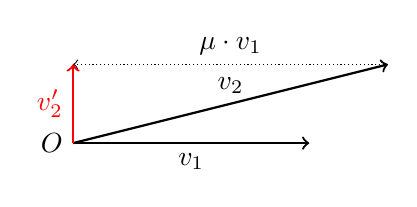
\begin{tikzpicture}
        \draw[->, thick](0,0) node[left]{$O$} -- node[above]{$\bvec{v}_2$} (4, 1);
        \draw[->, thick](0,0) -- node[below]{$\bvec{v}_1$} (3, 0);
        \draw[->, densely dotted](4,1) -- node[above]{$\mu\cdot \bvec{v}_1$} (0,1);
        \draw[->, thick, red](0,0) -- node[left, red]{$\bvec{v}_2'$} (0,1);
    \end{tikzpicture}
\end{center}

Using Gram-Schmidt, we have $\bvec{v}_2' = \bvec{v}_2 - \mu\cdot \bvec{v}_1$ where $\mu = \frac{\bvec{v}_1\cdot \bvec{v}_2}{\bvec{v}_1\cdot \bvec{v}_1}$.

With lattice reduction, we round $\mu$ to subtract by an integer multiple of $\bvec{v}_2$ instead.

\begin{center}
    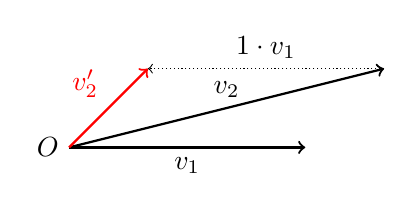
\begin{tikzpicture}
        \draw[->, thick](0,0) node[left]{$O$} -- node[above]{$\bvec{v}_2$} (4, 1);
        \draw[->, thick](0,0) -- node[below]{$\bvec{v}_1$} (3, 0);
        \draw[->, densely dotted](4,1) -- node[above]{$1\cdot \bvec{v}_1$} (1,1);
        \draw[->, thick, red](0,0) -- node[above left, red]{$\bvec{v}_2'$} (1,1);
    \end{tikzpicture}
\end{center}

Lattice reduction gives us
\[\bvec{v}_2' = \bvec{v}_2 - \lfloor\mu\rceil\cdot \bvec{v}_1\]

We do this again and again.

Code in \textsf{lattices.ipynb}.

We should prove that this gives us a reasonable basis when this algorithm finishes.
\begin{proposition}
    This algorithm terminates.
\end{proposition}
\begin{proof}
    Integer vectors $||\bvec{v}_1||$ and $||\bvec{v}_2||$ always decrease, and there are only \emph{finitely many} lattice vectors that strictly decrease.
\end{proof}

\begin{proposition}
    When this algorithm terminates, $\bvec{v}_1$ is the shortest vector in the lattice.
\end{proposition}
\begin{proof}
    At the end, we know that $||\bvec{v}_2||\geq ||\bvec{v}_1||$ and that
    \[-\frac{1}{2}\leq \mu = \frac{\bvec{v}_1\cdot \bvec{v}_2}{\bvec{v}_1\cdot \bvec{v}_1} \leq \frac{1}{2}.\]
    Any vector $\bvec{w} = a_1\bvec{v}_1 + a_2\bvec{v}_2$. So
    \begin{align*}
        ||\bvec{w}||^2 & = a_1^2\cdot ||\bvec{v}_1||^2 + 2a_1a_2(\bvec{v}_1\cdot \bvec{v}_2) + a_2^2||\bvec{v}_2||^2 \\
                       & \geq a_1^2\cdot ||\bvec{v}_1||^2 + a_1a_2||\bvec{v}_1||^2 + a_2^2||\bvec{v}_2||^2           \\
                       & = (a_1^2 + a_1a_2 + a_2^2)||\bvec{v}_1||^2
    \end{align*}
    And $a_1^2 + a_1a_2 + a_2^2 = \frac{3}{4}(a_1 - a_2)^2 + \frac{1}{4}(a_1 + a_2)^2 > 0$. \textsc{otoh} $a_1, a_2\in\ZZ$ so $a_1^2 + a_1a_2 + a_2^2\geq 1$.

    So any $||\bvec{w}||^2 \geq ||\bvec{v}_1||^2$.
\end{proof}